\section{Phân tích thực nghiệm các quyết định thiết kế mô hình}
\label{sec:thuc_nghiem_thiet_ke}

Để xác nhận tính tối ưu của kiến trúc mạng nơ-ron tự mã hóa Ba trạng thái, hệ thống thực hiện các thí nghiệm bổ sung nhằm làm rõ vai trò của từng thành phần kỹ thuật.

\subsection{Lựa chọn kiến trúc mạng qua các giai đoạn thử nghiệm}

Trước khi chốt kiến trúc cuối cùng, đồ án đã thử nghiệm ba cấu trúc mạng ở giai đoạn mô phỏng trên Kaggle: Vanilla AE làm mốc cơ sở, 1D-CNN AE cho dữ liệu chuỗi thời gian và LSTM AE cho phụ thuộc thời gian dài. Các mô hình được đánh giá trên cùng tập dữ liệu đã tiền xử lý, cùng quy trình huấn luyện và cùng các tiêu chí gồm sai số tái tạo, dung lượng mô hình sau khi nén INT8 trên Kaggle, độ trễ suy luận mô phỏng trên Kaggle và độ bất ổn khi thêm nhiễu. Kết quả ban đầu cho thấy thứ tự hiệu quả là 1D-CNN AE, Vanilla AE và LSTM AE.

\begin{table}[H]
\centering
\caption[So sánh ba kiến trúc mạng sau nén INT8 trên Kaggle]{So sánh ba kiến trúc mạng ở giai đoạn mô phỏng sau khi nén INT8 trên Kaggle. Các giá trị trong bảng là số liệu mô phỏng, chưa phải kết quả đo trực tiếp trên phần cứng thực tế.}
\label{tab:network_architecture_comparison}
\renewcommand{\arraystretch}{1.15}
\begin{tabular}{lccc}
\toprule
\textbf{Chỉ số} & \textbf{Vanilla AE} & \textbf{1D-CNN AE} & \textbf{LSTM AE} \\
\midrule
RAE Loss (MSE) & $0{,}004947$ & \textbf{$0{,}003698$} & $0{,}004198$ \\
Dung lượng INT8 (KB) & $375{,}01$ KB & $30{,}52$ KB & $368{,}66$ KB \\
Độ trễ mô phỏng (ms/Kaggle) & $76{,}56$ ms & $79{,}73$ ms & $129{,}50$ ms \\
Bất ổn với nhiễu (\%) & $793{,}63\%$ & \textbf{$706{,}43\%$} & $722{,}42\%$ \\
\bottomrule
\end{tabular}
\end{table}

Từ Bảng~\ref{tab:network_architecture_comparison}, 1D-CNN AE là ứng viên tốt nhất ở giai đoạn mô phỏng vì đạt sai số tái tạo thấp nhất, dung lượng sau nén INT8 nhỏ nhất và độ bất ổn với nhiễu thấp nhất trong ba mô hình. Vanilla AE có độ trễ mô phỏng thấp hơn 1D-CNN AE một chút nhưng lại có sai số tái tạo, dung lượng INT8 và độ bất ổn với nhiễu cao hơn đáng kể. LSTM AE không phù hợp với yêu cầu nhúng do độ trễ mô phỏng cao nhất và dung lượng sau nén vẫn lớn.

Mặc dù 1D-CNN AE đứng đầu ở giai đoạn mô phỏng, quá trình triển khai thực tế trên TensorFlow Lite Micro cho thấy kiến trúc này không ổn định khi đưa xuống phần cứng. Nguyên nhân chính gồm sai lệch kết quả giữa triển khai Conv1D trên Python và C++, yêu cầu đầu vào dạng chuỗi làm tăng chi phí quản lý bộ đệm, và rủi ro mất ổn định khi chuyển toàn bộ mô hình sang INT8. Vì vậy, đồ án chuyển hướng sang Symmetric Dense AE kết hợp khối trích xuất đặc trưng DSP 19 chiều. Phương án này không phải là mô hình đứng đầu trong vòng so sánh mô phỏng ban đầu, mà là quyết định thiết kế sau khi cân nhắc đầy đủ tính khả thi triển khai trên vi điều khiển Seeed Studio XIAO ESP32-S3.

Sau khi tối ưu, kiến trúc Symmetric Dense AE sử dụng cấu trúc đối xứng $19 \rightarrow 128 \rightarrow 64 \rightarrow 32 \rightarrow 64 \rightarrow 128 \rightarrow 19$ với lớp thắt cổ chai Sigmoid, tương thích tốt với lượng tử hóa INT8. Tổng dung lượng ba mô hình cho ba pha vận hành là $95{,}3$ KB, độ trễ suy luận trung bình đo thực tế đạt $6{,}4$ ms, đáp ứng yêu cầu triển khai nhúng và được chọn cho hệ thống cuối cùng.

\subsection{Nghiên cứu thành phần các biến thể mô hình}
So sánh giữa mô hình ba trạng thái đề xuất với các biến thể cấu hình khác nhau giúp xác định hiệu quả của từng thành phần. Kết quả được tổng hợp trong Bảng~\ref{tab:ablation_study}.

\begin{table}[H]
\centering
\caption[So sánh hiệu năng các biến thể mô hình]{So sánh hiệu năng giữa các biến thể mô hình trong nghiên cứu thành phần. (*) Trễ trung bình đo thực tế trên vi điều khiển Seeed Studio XIAO ESP32-S3 với N=1\,000 lần.}
\label{tab:ablation_study}
\begin{adjustbox}{max width=\textwidth}
\begin{tabular}{|l|c|c|c|c|}
\hline
\textbf{Biến thể} & \textbf{MAE (SPIN)} & \textbf{F1-Score} & \textbf{Trễ ($ms$)} & \textbf{Model Flash (KB)} \\ \hline
Mô hình đơn AE (Chung 3 pha) & 0,0421 & 0,845 & 6,5 & 31,7 \\ \hline
Ba trạng thái AE (Không dùng MAE có trọng số) & 0,0291 & 0,912 & 6,4* & 95,3 \\ \hline
\textbf{Ba trạng thái AE đề xuất} & \textbf{0,0242} & \textbf{0,9967} & \textbf{6,4*} & \textbf{95,3} \\ \hline
\end{tabular}
\end{adjustbox}
\end{table}

Kiến trúc Ba trạng thái đem lại bước nhảy lớn nhất về hiệu năng. Biến thể mô hình đơn sử dụng chung một mô hình cho cả 3 pha chỉ đạt F1-Score 0,845, thấp hơn đáng kể so với Ba trạng thái, cho thấy mỗi pha có đặc tính thống kê riêng biệt. Bên cạnh đó, hàm mất mát MAE có trọng số (trọng số rung động gấp 5 lần âm thanh) nâng F1 từ 0,912 lên 0,9967 ở pha SPIN, khẳng định tầm quan trọng của việc ưu tiên kênh cảm biến mang tính vật lý cao hơn.

Kích thước lớp thắt cổ chai ảnh hưởng trực tiếp đến khả năng nén đặc trưng và tài nguyên tính toán. Khảo sát các kích thước tiềm năng tìm ra kích thước tối ưu (Bảng~\ref{tab:bottleneck_sweep}).

\begin{table}[H]
\centering
\caption[Kết quả khảo sát lớp thắt cổ chai]{Kết quả khảo sát kích thước lớp thắt cổ chai. \textit{Lưu ý: Các giá trị độ trễ (ms) trong bảng là ước tính tương đối dùng để so sánh tỷ lệ tài nguyên.}}
\label{tab:bottleneck_sweep}
\begin{tabular}{|c|c|c|c|c|}
\hline
\textbf{Số chiều} & \textbf{MAE (TB)} & \textbf{Tham số} & \textbf{Trễ ($ms$)} & \textbf{Đánh giá} \\ \hline
8 & 0,0321 & 19.347 & 5,8 & Underfitting \\ \hline
16 & 0,0265 & 22.563 & 6,1 & Đạt yêu cầu \\ \hline
\textbf{32} & \textbf{0,0242} & \textbf{25.779} & \textbf{6,4} & \textbf{Điểm tối ưu} \\ \hline
64 & 0,0241 & 32.211 & 7,4 & Bão hòa \\ \hline
\end{tabular}
\end{table}

Tại 32 chiều, mô hình đạt hiệu năng tối ưu. Tăng lên 64 chiều chỉ giảm sai số MAE không đáng kể nhưng tăng 15\% độ trễ suy luận và dung lượng bộ nhớ. 32 chiều là lựa chọn tối ưu cho vi điều khiển Seeed Studio XIAO ESP32-S3.

\subsection{Phân tích ngưỡng $\tau$ bằng đường cong ROC và chỉ số Youden's J}
Phân tích đường cong ROC tối ưu hóa khả năng phân tách giữa dữ liệu bình thường và bất thường (Hình~\ref{fig:roc_all_states}).

\begin{figure}[H]
    \centering
    \begin{subfigure}{0.32\textwidth}
        \centering
        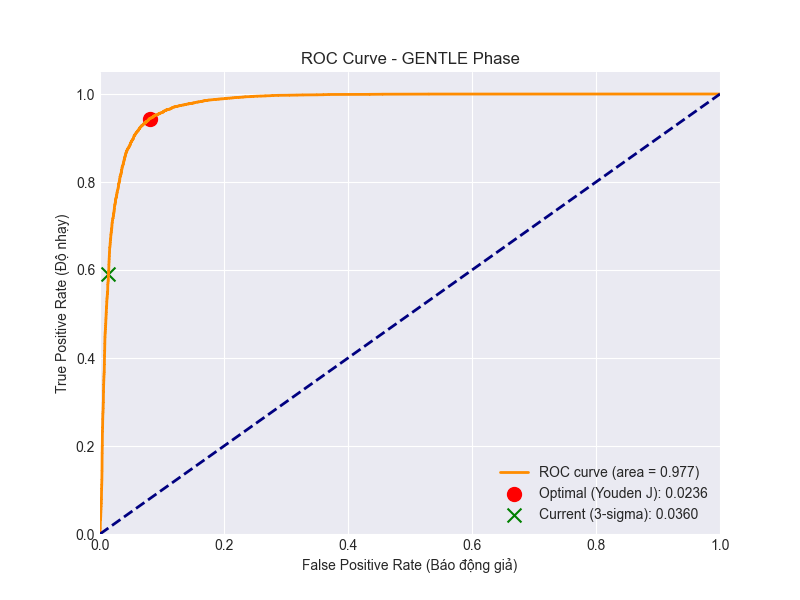
\includegraphics[width=\linewidth]{chap4/image/roc_gentle.png}
        \caption{GENTLE}
    \end{subfigure}
    \hfill
    \begin{subfigure}{0.32\textwidth}
        \centering
        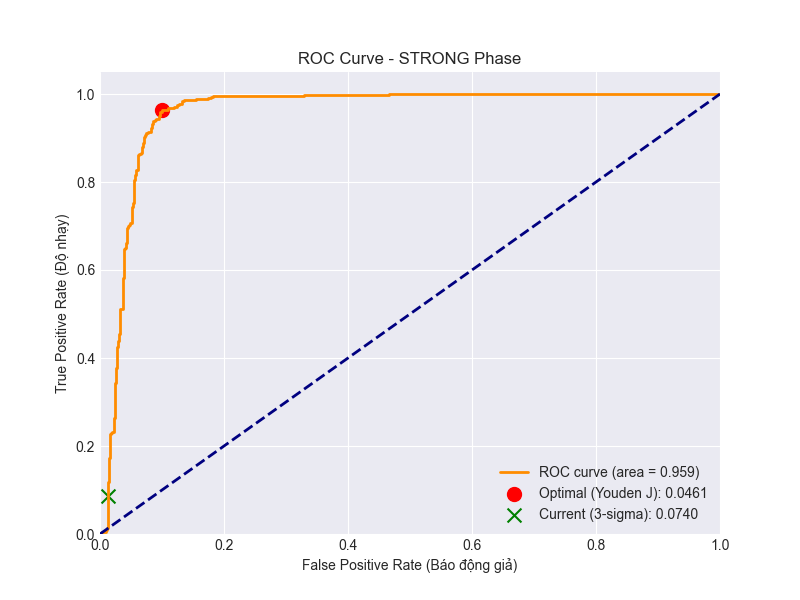
\includegraphics[width=\linewidth]{chap4/image/roc_strong.png}
        \caption{STRONG}
    \end{subfigure}
    \hfill
    \begin{subfigure}{0.32\textwidth}
        \centering
        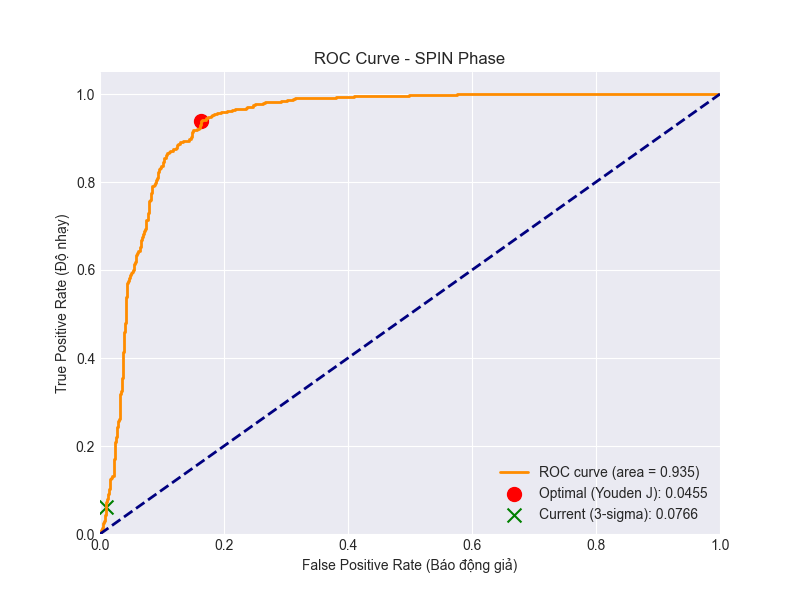
\includegraphics[width=\linewidth]{chap4/image/roc_spin.png}
        \caption{SPIN}
    \end{subfigure}
    \caption[Đường cong ROC ba pha vận hành]{Đường cong ROC và điểm Youden's J Index tối ưu cho ba pha vận hành GENTLE, STRONG và SPIN.}
    \label{fig:roc_all_states}
\end{figure}

Diện tích dưới đường cong (AUC) đạt: GENTLE (0,9989), STRONG (0,9837), SPIN (0,9993). Thông qua chỉ số Youden's J ($J = Sensitivity + Specificity - 1$), chúng tôi xác định ngưỡng $\tau_{optimal}$. Tuy nhiên, trong thiết kế thực tế, hệ thống ưu tiên ngưỡng thống kê $3\sigma$ (nghiêm ngặt hơn Youden) để giảm cảnh báo giả và tránh ảnh hưởng tiêu cực đến người dùng trong môi trường dân dụng.

Tại ngưỡng $3\sigma$, độ chính xác (Precision) đạt 0,99 ở cả 3 pha, nhưng chỉ số Recall ở pha GENTLE giảm xuống 0,78 so với 0,91 tại điểm Youden. Đây là sự đánh đổi kỹ thuật nhằm đảm bảo độ ổn định của hệ thống cảnh báo trước các nhiễu môi trường.

\subsection{Phân tích sâu nguyên nhân sai số pha GENTLE}
Pha STRONG có AUC thấp nhất (0,9837), trong khi pha GENTLE vẫn là chế độ dễ phát sinh nhiễu nền do cường độ vận hành thấp. Phân tích các mẫu bị nhận diện sai cho thấy hai vấn đề chính:

\begin{itemize}
    \item \textbf{False Negatives:} Xảy ra khi biến động gia tốc trục Z cực nhỏ (MAE xấp xỉ ngưỡng bình thường). Ở mức năng lượng này, đặc trưng rung động của lỗi bị lấn át bởi nhiễu nền của động cơ Inverter, khiến mạng nơ-ron tự mã hóa tái tạo lỗi như tín hiệu bình thường.
    \item \textbf{False Positives:} Chủ yếu do các nhiễu âm thanh đột biến từ môi trường bên ngoài (tiếng va chạm vật lý vào vỏ máy) không thuộc chu kỳ vận hành của máy giặt nhưng trùng vào dải tần số bộ lọc Mel mà mô hình giám sát.
\end{itemize}
